\documentclass[10pt,svgnames,usenames,table]{beamer}
\usetheme{metropolis}
\usepackage[math]{iwona}
\usepackage{scalerel}
\def\lVert{\mid\!\mid}
\def\rVert{\mid\!\mid}

\usepackage{custom}
\usepackage{tikz}
\usepackage{tkz-graph}
\usetikzlibrary{arrows}
\usepackage{readarray}
\usepackage{nsi}



\newcommand\Wider[2][3em]{%
\makebox[\linewidth][c]{%
  \begin{minipage}{\dimexpr\textwidth+#1\relax}
  \raggedright#2
  \end{minipage}%
  }%
}

\title{Parallel optimization on the Entropic Cone}
\date{}
\author{Beno\^it Legat \and Rapha\"el M. Jungers}
\institute{Universit\'e catholique de Louvain (UCL)}

\begin{document}
  \maketitle

  \begin{frame}
    \frametitle{Shannon's Entropy}
    \begin{block}{Univariate}
      Discrete random variable $X$ taking values
      in $\mathcal{X}$.

      Shannon's entropy:
      \[ H(X) = \sum_{x \in \mathcal{X}} \Pr[X = x] \log\frac{1}{\Pr[X = x]} \]
    \end{block}
    \begin{block}{Multivariate}
      Random variables $X = (X_1, \ldots, X_n)$.

      Joint Shannon's entropy: Given $\Jis \subseteq [n] = \{1, \ldots, n\}$,
      \[ h_{\Jis} \eqdef H(X_\Jis) = \sum_{x \in \mathcal{X}_\Jis} \Pr[X_\Jis = x] \log \frac{1}{\Pr[X_\Jis = x]}. \]
    \end{block}
  \end{frame}

  \begin{frame}
    \frametitle{Entropy Vector}
    \latthreenb{$H(X_1)$ $H(X_2)$ $H(X_1,X_2)$ $H(X_3)$ $H(X_1,X_3)$ $H(X_2,X_3)$ $H(X_1,X_2,X_3)$}
  \end{frame}

  \begin{frame}
    \frametitle{Example: One Time Pad}
    \[ \mathsf{plaintext} \oplus \mathsf{key} = \mathsf{ciphertext}. \]
    \latthreenb{1 1 2 1 2 2 2}
  \end{frame}

  \begin{frame}
    \frametitle{Shannon's inequality}
    {\only<2,3>{\em}\only<1>{\bf}Normalization:}
    \[ h_{\emptyset} = 0 \]
    {\only<1,3>{\em}\only<2>{\bf}Nondecreasing:}
    If $\Iis \subseteq \Jis$ then
    \[ h_{\Iis} \leq h_{\Jis} \]
    {\only<1,2>{\em}\only<3>{\bf}Submodular:}
    For any $\Jis, \Kis$,
    \[ h_{\Jis} + h_{\Kis} \geq h_{\Jis \cup \Kis} + h_{\Jis \cap \Kis} \]
    \begin{center}
      \begin{tikzpicture}[x=1.5cm,y=1cm]
        \tikzset{VertexStyle/.style = {
        shape = rectangle}}
        \only<2,3>{
          \Vertex[x=1, y=0,L={000 0}]{000}
        }
        \only<1>{
          \Vertex[x=0, y=1,L={001 1}]{001}
        }
        \Vertex[x=1, y=1,L={010 1}]{010}
        \Vertex[x=2, y=1,L={100 1}]{100}
        \only<1>{
          \Vertex[x=0, y=2,L={011 2}]{011}
        }
        \Vertex[x=1, y=2,L={101 2}]{101}
        \Vertex[x=2, y=2,L={110 2}]{110}
        \only<1,2>{
          \Vertex[x=1, y=3,L={111 2}]{111}
          \Vertex[x=1, y=2,L={101 2}]{101}
        }
        \tikzset{VertexStyle/.append style = {
        color = blue}}
        \only<1>{
          \Vertex[x=1, y=0,L={000 0}]{000}
        }
        \only<2,3>{
          \Vertex[x=0, y=2,L={011 2}]{011}
        }
        \only<3>{\Vertex[x=1, y=2,L={101 2}]{101}}
        \tikzset{VertexStyle/.append style = {
        color = red}}
        \only<2,3>{
          \Vertex[x=0, y=1,L={001 1}]{001}
        }
        \only<3>{
          \Vertex[x=1, y=3,L={111 2}]{111}
        }

        \Edge(000)(100)
        \Edge(000)(010)
        \Edge(000)(001)


        \Edge(100)(110)
        \Edge(100)(101)

        \Edge(010)(110)
        \Edge(010)(011)

        \Edge(001)(101)
        \Edge(001)(011)


        \Edge(110)(111)
        \Edge(101)(111)
        \Edge(011)(111)
      \end{tikzpicture}
    \end{center}
    \only<2,3>{\[\text{\color{blue}blue} \geq \text{\color{red}red}\]}
    \only<1>{\[\text{\color{blue}blue} = 0\]}
  \end{frame}

  \begin{frame}{Non-Shannon inequalities}
    \metroset{block=fill}
    \begin{block}{Entropic cone $\Ec$}
      Set of vectors $h$ that are the entropy vector of $n$ jointly distributed random variables.

      [Zhang, Yeung 1997]: $\cEc$ is a cone.
    \end{block}
    \begin{block}{Shannon cone/polymatroid cone $\Pm$}
      Set of vectors $h$ that satisfies all shannon's inequalities.
    \end{block}
    \begin{block}{Non-Shannon inequalities}
      Inequalities valid for $\cEc$ but not for $\Pm$.
    \end{block}

    Does $\cEc = \Pm$ or are there non-Shannon inequalities ?
  \end{frame}

  \begin{frame}
    \frametitle{First non-Shannon inequalities [Zhang, Yeung 1998]}
    Non-entropic vector satisfying Shannon's inequalities:
    \latfournb[1.5]{2 2 3 2 3 3 4 2 3 3 4 4 4 4 4}
  \end{frame}

  \begin{frame}
    \frametitle{How many non-Shannon inequalities ?}
    \begin{block}{[\matus{} 2007]}
      The cone $\cEc$ is not polyhedral.

      Polyhedral convex set: finite intersection of half-spaces.
      \[ \bigcap \{\, x \mid \la a, x \ra \leq \beta \,\} \]
    \end{block}
    \begin{block}{[Mejia and Montoya 2015]}
      The cone $\cEc$ is not semialgebraic.

      Algebraic convex set: finite intersection of sets defined by a polynomial inequality
      \[ \bigcap \{\, x \mid p(x) \leq \beta \,\} \]
      Semialgebraic convex set: projection of algebraic set.
    \end{block}
  \end{frame}

  \begin{frame}
    \frametitle{Generating non-Shannon inequalities : Inner-Adhesivity}

    Given $n$ jointly distributed random variables of probability mass function $p$,
    we can generate the following new probability mass function for any $\Jis$, $\Kis$, $\Iis = \Jis \cap \Kis$:
    \[ \frac{p_{\Jis}(x_{\Jis})p_{\Kis}(x_{\Kis})}{p_{\Iis}(x_{\Iis})} = p_{\Jis|\Iis}(x_{\Jis}|x_{\Iis})p_{\Kis|\Iis}(x_{\Kis}|x_{\Iis})p_{\Iis}(x_{\Iis}) \]
    \uncover<2,3>{
      Let's try it with $\textcolor{red}{\Jis = 011}$ and $\textcolor{blue}{\Kis = 110}$ (so $\textcolor{purple}{\Iis = 010}$).

      \begin{center}
        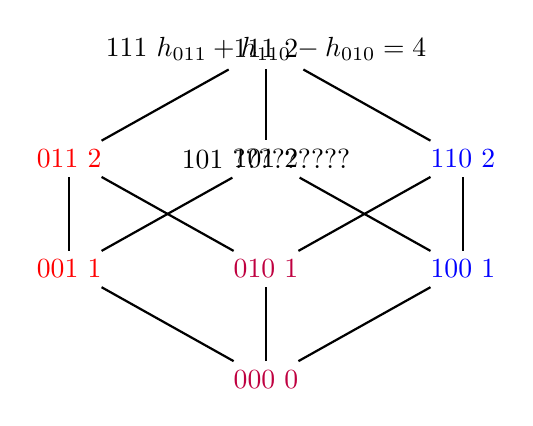
\begin{tikzpicture}[x=2.5cm,y=1.4cm]
          \tikzset{VertexStyle/.style = {
          shape = rectangle}}
          \uncover<2>{\Vertex[x=1, y=2,L={101 2}]{101}}
          \uncover<3>{\Vertex[x=1, y=2,L={101 ?????????}]{101}}
          \uncover<2>{\Vertex[x=1, y=3,L={111 2}]{111}}
          \uncover<3>{\Vertex[x=1, y=3,L={111 $h_{011} + h_{110} - h_{010}=4$}]{111}}
          \tikzset{VertexStyle/.append style = {
          color = red}}
          \Vertex[x=0, y=2,L={011 2}]{011}
          \Vertex[x=0, y=1,L={001 1}]{001}
          \tikzset{VertexStyle/.append style = {
          color = blue}}
          \Vertex[x=2, y=2,L={110 2}]{110}
          \Vertex[x=2, y=1,L={100 1}]{100}
          \tikzset{VertexStyle/.append style = {
          color = purple}}
          \Vertex[x=1, y=0,L={000 0}]{000}
          \Vertex[x=1, y=1,L={010 1}]{010}

          \Edge(000)(100)
          \Edge(000)(010)
          \Edge(000)(001)

          \Edge(100)(110)
          \Edge(100)(101)

          \Edge(010)(110)
          \Edge(010)(011)

          \Edge(001)(101)
          \Edge(001)(011)

          \Edge(110)(111)
          \Edge(101)(111)
          \Edge(011)(111)
        \end{tikzpicture}
      \end{center}
    }
  \end{frame}
  \begin{frame}
    \frametitle{Generating non-Shannon inequalities : Self-Adhesivity}
    Given $n$ jointly distributed random variables of probability mass function $p$,
    we can generate the following new probability mass function for any $\Iis \subseteq \Jis$,
    \[ \frac{p_{\Jis'}(x_{\Jis'})p_{\Jis}(x_{\Kis})}{p_{\Iis}(x_{\Iis})} = p_{\Jis'|\Iis}(x_{\Jis'}|x_{\Iis})p_{\Jis|\Iis}(x_{\Kis}|x_{\Iis})p_{\Iis}(x_{\Iis}), \]
    where $n' = n + |\Jis \setminus \Iis|$, $\Jis' = [n]$ and $\Kis = ([n'] \setminus [n]) \cup \Iis$.
    \uncover<2->{
      Let's try it with $\textcolor{red}{\Jis = 11}$ and $\textcolor{purple}{\Iis = 10}$ (so $n' = 3$, $\Jis' = 011$, $\textcolor{blue}{\Kis = 110}$).

      \begin{center}
        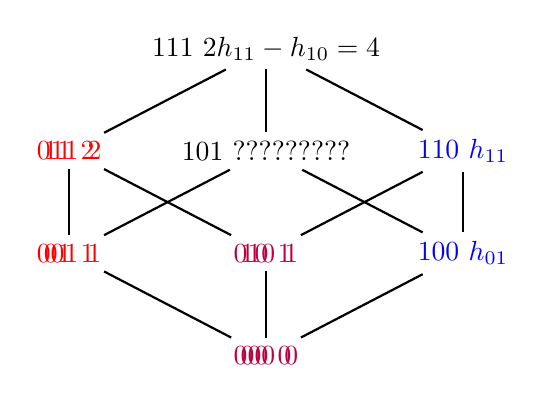
\begin{tikzpicture}[x=2.5cm,y=1.3cm]
          \tikzset{VertexStyle/.style = {
          shape = rectangle}}
          \uncover<4>{\Vertex[x=1, y=2,L={101 ?????????}]{101}}
          \uncover<4>{\Vertex[x=1, y=3,L={111 $2h_{11} - h_{10}=4$}]{111}}
          \tikzset{VertexStyle/.append style = {
          color = red}}
          \uncover<2>{
            \Vertex[x=0, y=2,L={11 2}]{011}
            \Vertex[x=0, y=1,L={01 1}]{001}
          }
          \uncover<3->{
            \Vertex[x=0, y=2,L={011 2}]{011}
            \Vertex[x=0, y=1,L={001 1}]{001}
          }
          \tikzset{VertexStyle/.append style = {
          color = blue}}
          \uncover<3->{\Vertex[x=2, y=2,L={110 $h_{11}$}]{110}}
          \uncover<3->{\Vertex[x=2, y=1,L={100 $h_{01}$}]{100}}
          \tikzset{VertexStyle/.append style = {
          color = purple}}
          \uncover<2>{
            \Vertex[x=1, y=0,L={00 0}]{000}
            \Vertex[x=1, y=1,L={10 1}]{010}
          }
          \uncover<3->{
            \Vertex[x=1, y=0,L={000 0}]{000}
            \Vertex[x=1, y=1,L={010 1}]{010}
          }

          \Edge(000)(010)
          \Edge(000)(001)

          \Edge(010)(011)

          \Edge(001)(011)

          \uncover<3->{
            \Edge(100)(110)
            \Edge(000)(100)

            \Edge(010)(110)
          }
          \uncover<4>{
            \Edge(100)(101)
            \Edge(001)(101)
            \Edge(110)(111)
            \Edge(101)(111)
            \Edge(011)(111)
          }
        \end{tikzpicture}
      \end{center}
    }
  \end{frame}
  \begin{frame}{Structure of the adhesivity invariance}
    If $h \in \Ec$ then there exists $g \in \Ec[n']$ such that $\forall \Iis \subseteq \Lis \subseteq \Jis' \cup \Kis$
    \[ g_{\Lis} = h_{\Lis \cap \Jis'} + h_{\Lis \cap \Kis} - h_{\Iis} \]
    If $\Iis \not\subseteq \Lis$, $g_{\Lis}$ is \emph{free} !

    \uncover<2->{
      To generate non-Shannon inequalities, we use the fact that these $g_{\Lis}$ \emph{exists} and $g$ is also entropic,
      so $g \in \Pm[n']$ and we can enforce adhesivity invariance on $g$ too.
    }

    \uncover<3>{
      The adhesivity invariance is linear:
      Each adhesivity can be modeled by
      \[ \exists g \in \Ec[n'] \text{ such that } Wg = Th \]
      for some matrix $W,T$.
    }
  \end{frame}

  \begin{frame}{Stochastic Programming}
    Markov chain of linear programs.
    Linear program at state $u$:
    \begin{align*}
      Q(x, u) = \mini\,\, & c^T y + \mathcal{Q}_u(y)\\
      \text{s.t.} \,& W_u y = h_u - T_ux,\\
                    & x \geq 0.
    \end{align*}
    where $\mathcal{Q}_u(y)$ is the sum of $Q(x, v)$ for each state $v$ accessible from $u$
    weighted by the probability to go from state $u$ to state $v$.

    \uncover<2>{If it is infeasible, $Q(x, u) = +\infty$.}
  \end{frame}
  \begin{frame}{Stochastic Program for the Entropic Cone}
    Linear Program at initial state:
    \begin{align*}
      \mini\,\, & c^T h\only<1-2>{ + \mathcal{Q}_0(h)}\only<3-4>{ + \mathcal{Q}_{n_0}(h)}\\
      \text{s.t.} \,& h \in \Pm[n_0]\only<1-4>{.}
      \uncover<5>{
        \\
        & h \in \dom(\mathcal{Q}_{n_0}).
      }
    \end{align*}

    Linear Program for each adhesivity $\mathsf{a}$:
    \begin{align*}
      Q(h, (n, \mathsf{a})) = \mini\,\, & \only<1-2>{\mathcal{Q}_{(n, \mathsf{a})}(g)}\only<3-4>{\mathcal{Q}_{n'}(g)}\only<5>{0}\\
      \text{s.t.} \,& g \in \mathsf{a}(h)\\\
                    & g \in \Pm[n']\only<1-4>{.}
      \uncover<5>{
        \\
        & g \in \dom(\mathcal{Q}_{n'}).
      }
    \end{align*}
    \uncover<2->{This state is accessible for all linear programs of dimension $2^n-1$ so $\mathcal{Q}_{(n, \mathsf{a})}$ only depends on $n'$.}

    \uncover<4->{The function $\mathcal{Q}_n$ is either $0$ or $+\infty$.}
  \end{frame}

  \begin{frame}{Polyhedral approximation of $\dom(\mathcal{Q}_n)$}
    Linear Program at initial state:
    \begin{align*}
      \mini\,\, & c^T h\\
      \text{s.t.} \,& h \in \Pm[n_0]\\
      \only<1>{
        & h \in \dom(\mathcal{Q}_{n_0}).
      }
      \only<2->{
                    & D_{n_0}h \leq d_{n_0}.
      }
    \end{align*}

    Linear Program for each adhesivity $\mathsf{a}$:
    \begin{align*}
      Q(h, (n, \mathsf{a})) = \mini\,\, & 0\\
      \text{s.t.} \,& g \in \mathsf{a}(h)\\\
                    & g \in \Pm[n']\\
      \only<1>{
        & g \in \dom(\mathcal{Q}_{n'}).
      }
      \only<2->{
        & D_{n'}g \leq d_{n'}.
      }
    \end{align*}

      The domain of $\mathcal{Q}_n$ is approximated by the polyhedron
    \[ \{\, x \mid D_n x \leq d_n \,\}. \]
    \uncover<3>{Program at state $(n,\mathsf{a})$ is infeasible $\to$ unbouded ray of the dual $\to$ new cut for $D_n, d_n$.}
  \end{frame}
  \begin{frame}{Stochastic Dual Dynamic Programming}
    \begin{algorithmic}
      \FOR{$k = 1,2,\ldots,K$}
      \STATE Pick a set $P$ of paths of length $m$ starting at the initial state.
      \STATE Solve the optimization program
      \begin{align*}
        \mini\,\, & c(h)\\
        \text{s.t.} \,& h \in \Pm[n_0] \cap \mathbb{F} \cap \dom(\mathcal{Q}_0),
      \end{align*}
      \FOR{$i = 1,2,\ldots,m$}
      \FORALL{$p \in P$}
      \STATE Solve $Q(h, (n_{p,i}, \mathsf{a}_{p,i}))$ where $h$ is the optimal solution of the previous state in the path.
      \IF{the program is infeasible}
      \STATE Add a feasibility cut for $\dom(Q(\cdot, (n_{p,i}, \mathsf{a}_{p,i})))$
      \STATE Remove $p$ from $P$
      \ENDIF
      \ENDFOR
      \ENDFOR
      \ENDFOR
    \end{algorithmic}
  \end{frame}

  \begin{frame}{Ingleton score}
    \[ \ingsc \eqdef \inf_{0 \neq h \in \Ec[4]} \ingij{i}{j}(h) \]
    where $\ingij{i}{j}(h) = \la \ingsq{i}{j}, h \ra / h_{[n]}$ and $\ingsq{i}{j}$ is the Ingleton dual entropy vector.
    \begin{block}{[Dougherty et al. 2011]}
      \[ -0.15789 \leq \ingsc. \]
    \end{block}
    \begin{block}{[\matus{} and Csirmaz 2013]}
      \[ \ingsc \leq -0.09243. \]
    \end{block}
  \end{frame}

  \begin{frame}{Attacking the Ingleton score}
    \begin{block}{Only self-adhesivity, $n \leq 7$ and $m \leq 2$}
      \[ -0.15854 \leq \ingsc. \]
    \end{block}
    \uncover<2->{
      \begin{block}{Only self-adhesivity, $n \leq 8$ and $m \leq 3$}
        \[ -0.15789 \leq \ingsc. \]
      \end{block}
    }
    \uncover<3>{
      \begin{block}{Only self-adhesivity, $n \leq 9$ and $m \leq 4$}
        \emph{Stay tuned}.
      \end{block}
    }
  \end{frame}

  \begin{frame}{\jlpkg{EntropicCone} toolbox}
    \jlpkg{EntropicCone} : Optimization on and Approximation of the Entropic Cone.

    \begin{center}
      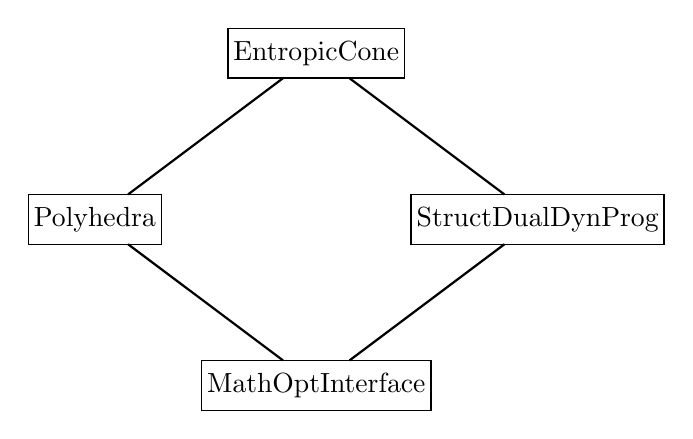
\begin{tikzpicture}[x=40,y=60]
        \SetVertexNormal[Shape=rectangle]
        \Vertex[x=0,y=0,L={\jlpkg{EntropicCone}}]{EC}
        \Vertex[x=-2,y=-1,L={\jlpkg{Polyhedra}}]{P}
        \Vertex[x=2,y=-1,L={\jlpkg{StructDualDynProg}}]{SDDP}
        \Vertex[x=0,y=-2,L={\jlpkg{MathOptInterface}}]{MOI}
        \Edge(EC)(P)
        \Edge(EC)(SDDP)
        \Edge(MOI)(P)
        \Edge(MOI)(SDDP)
      \end{tikzpicture}
    \end{center}
  \end{frame}

  \begin{frame}{Conclusion}
    \begin{itemize}
      \item Parallelizable optimization algorithm on the Entropic Cone.
      \item Possible to add nonlinear constraints and use nonlinear objective.
      \item Current best lower bound on $\ingsc$ obtained in under a minute.
    \end{itemize}
  \end{frame}
\end{document}
